\graphicspath{ {Figures/implementation/} }

\chapter{Υλοποίηση}\label{ch:Implementation}

\section{Αρχιτεκτονική του συστήματος}
Για την υλοποίηση του προτεινόμενου συστήματος αιμοδοσίας, χρησιμοποιείται η διαδεδομένη αρχιτεκτονική πολλαπλών επιπέδων (multitier architecture) όπως απεικονίζεται στο σχήμα \ref{fig:architect_schema}.

	\begin{figure}[H]
	    \centering
	    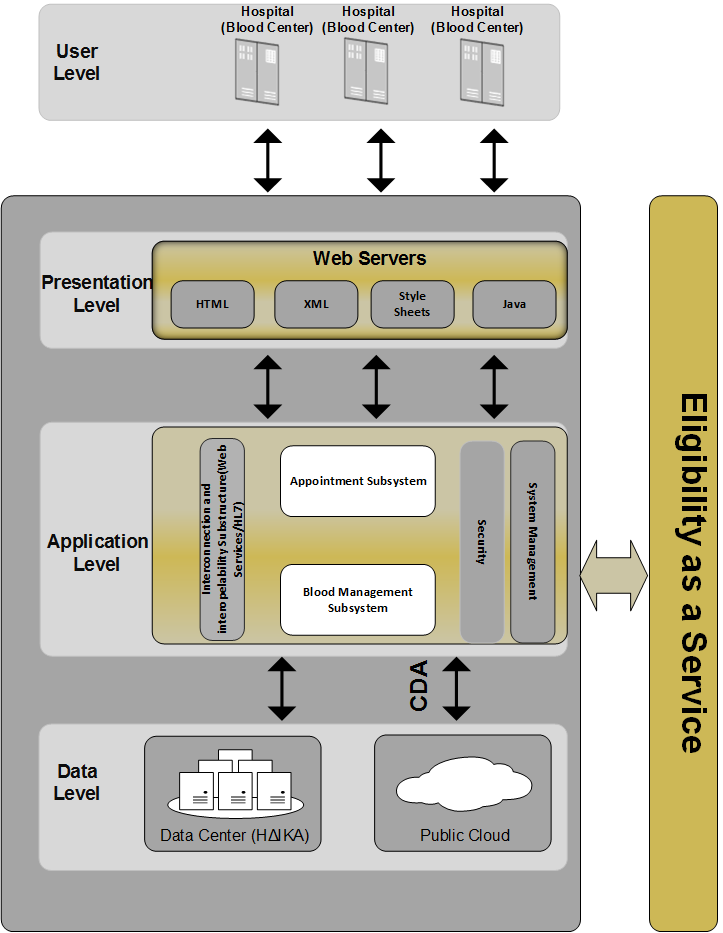
\includegraphics[width=1\textwidth]{architecture.png}
	    \caption{ Σχηματικό διάγραμμα του συστήματος. }
	    \label{fig:architect_schema}
	\end{figure}
	Τα επίπεδα που χρησιμοποιούνται στο σχήμα είναι τα εξής:
	\begin{itemize}
	\item Επίπεδο Βάσης Δεδομένων (Database layer). Στο επίπεδο αυτό τηρείται το σύνολο των επιχειρησιακών δεδομένων αλλά και των βοηθητικών αρχείων για την εύρυθμη λειτουργία των εφαρμογών του συστήματος.
	
	\item  Επίπεδο Επιχειρησιακής Λογικής (Bussiness logic layer). Στο επίπεδο αυτό διαμορφώνεται η επιχειρησιακή λογική ώστε να παραμετροποιείται το σύστημα με βάση τις ανάγκες λειτουργίας του φορέα.
	
	\item Επίπεδο Παρουσίασης ( Presentation layer). Αφορά στη διαπροσωπεία (User Interface) και στον τρόπο παρουσίασης των δεδομένων σύμφωνα με το ρόλο του κάθε χρήστη. Το προτεινόμενο σύστημα βασίζεται στις τεχνολογίες WEB και στις τεχνολογίες παρουσίασης του Android.
	
	\end{itemize}

\section{Βάση δεδομένων}
	\subsection{Σχήμα Βάσης}
	
	Στην ενότητα αυτή παρουσιάζεται το σχεσιακό διάγραμμα της βάσης NoSQL για το προτεινόμενο σύστημα ενώ παράλληλα αποτυπώνονται συνοπτικά οι προτεινόμενες δομές δεδομένων που υλοποιούν το προτεινόμενο σχήμα δεδομένων. Στο σχήμα \ref{fig:database_diag} απεικονίζεται η βάση δεδομένων.
	
	\begin{figure}[H]
	    \centering
	    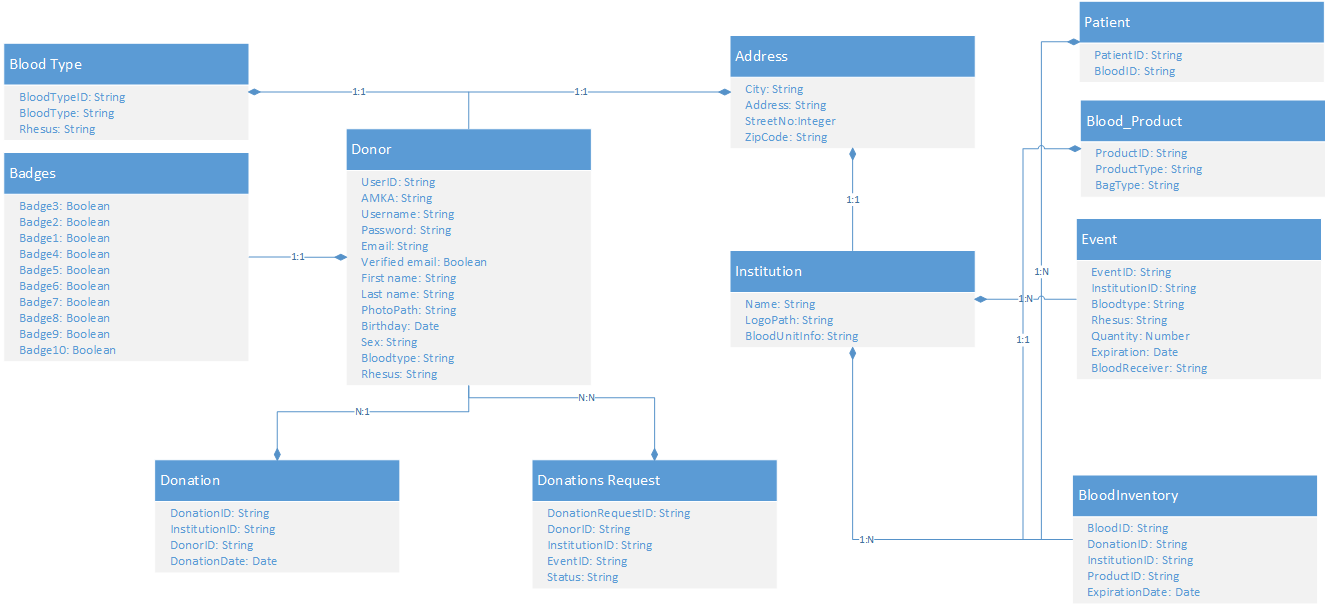
\includegraphics[width=1\textwidth]{Class_Diagram.png}
	    \caption{Σχεσιακό διάγραμμα της βάσης του συστήματος.}
	    \label{fig:database_diag}
	\end{figure}
	
		Κεντρικοί πίνακες είναι ο πίνακας Donor και ο πίνακας Institution. Ο πίνακας Donor περιέχει τα στοιχεία του εθελοντή αιμοδότη τα οποία είναι τα εξής: ΑΜΚΑ,όνομα, επώνυμο, photopath (για αποθήκευση φωτογραφίας), ημερομηνία γέννησης, φύλο, userid, username, password, e-mai, ημερομηνία δημιουργίας λογαριασμού. Ο πίνακας Institution περιέχει τα στοιχεία του κέντρου αιμοδοσίας, τα οποία είναι: userID,username, password, email, ημερομηνία δημιουργίας λογαριασμού, logopath, λοιπά στοιχεία του ινστιτούτου. Υπάρχει επιπλέον ο πίνακας Address ο οποίος περιέχει τα στοιχεία: πόλη, διεύθυνση, νούμερο και ταχυδρομικός κώδικας και ενώνεται με σχέση 1-1 με το κέντρο αιμοδοσίας και με σχέση 1-1 με τον εθελοντή αιμοδότη και ο πίνακας BloodType  ο οποίος αποθηκεύει ένα id για τον τύπο του αίματος, την ομάδα αίματος και το rhesus και συνδέεται με σχέση 1:1 με τον εθελοντή αιμοδότη.
	
		Ο πίνακας Donation περιεχέι στοιχεία για τις πραγματοποιηθείσες αιμοδοσίες, όπως: donationid, το id του κέντρου αιμοδοσίας στο οποίο έλαβαν χώρα, το id του εθελοντή και την ημερομηνία κατά την οποία πραγματοποιήθηκε η αιμοδοσία. Ο πίνακας Donation συνδέεται με σχέση N:1 με τον πίνακα Donor, καθώς ένας Donor μπορεί να έχει πραγματοποιήσει N αιμοδοσίες. Ο πίνακας DonationRequest περιέχει τα αιτήματα αιμοδοσίας που στέλνονται στους χρήστες, με τα εξής στοιχεία: το id του εθελοντή, το id του κέντρου αιμοδοσίας, το id του γεγονότος αιμοδοσίας στο οποίο αναφέρεται  και τέλος ένα πεδίο που λέγεται κατάσταση και περιγράφει την κατάσταση του αιτήματος (σε αναμονή, εγκεκριμένο, απορριφθέν ). Ο πίνακας DonationRequest ενώνεται με σχέση Ν:Ν με τους εθελοντές, καθώς πολλά αιτήματα αιμοδοσίας αντιστοιχούν σε πολλούς αιμοδότες.
	
		Στον πίνακα BloodProduct αποθηκεύονται στοιχεία για τα παράγωγα αίματος που προκύπτουν από κάποια αιμοδοσία, ενώ στον πίνακα Patient αποθηκεύονται στοιχεία για τον ασθενή στον οποίο καταλήγει το αίμα, και συσχετίζεται με σχέση 1-1 με τον πίνακα BloodInventory. Ο πίνακας BloodInventory αντιστοιχεί σε κάθε σακούλα αίματος που έχει περάσει εργαστηριακούς ελέγχους και έχει εγκριθεί και περιέχει στοιχεία: id του αίματος, id της αιμοδοσίας από την οποία προήλθε, το id του κέντρου αιμοδοτών, το id του αντικειμένου, ημερομηνία λήξης του αίματος. Τέλος, ο πίνακας badges περιέχει τις δέκα διαφορετικές κατηγορίες εμβλημάτων που μπορεί να κερδίσει ένας εθελοντής αιμοδότης και συνδέεται με σχέση 1:1 με τον εθελοντή αιμοδότη.

\section{Web App}
	\subsection{NodeJs - Server Establishment}
	
	Όπως αναφέρθηκε και στην ενότητα \ref{ssec:node} χρησιμοποιήσαμε την πλατφόρμα NodeJs για να αναπτύξουμε την εφαρμογή μας. Για να δουλέψουμε πάνω στο NodeJS χρησιμοποιούμε το το Express framework, εγκαθιστώντας το πακέτο Express από τον Node Package Manager (NPM) και συνέχεια ενσωματώνουμε το πακέτο Express. 
	
		\begin{lstlisting}[language=Javascript]	
	  		var express = require('express');
		\end{lstlisting}
		
		
	Αφού έχουμε εξάγει και ενσωματώσει το πακέτο Express δημιουργούμε ένα νέο Express αντικείμενο.	
		
		
		\begin{lstlisting}[language=Javascript]	
			var app = express(); 	
 		\end{lstlisting}
		
			Το αντικείμενο "app" που έχουμε φτιάξει ουσιαστικά ξεκινάει τον server μας και εμπεριέχει μεθόδους για 
			\begin{itemize}
			\item Να δρομολογεί HTTP αιτήσεις.
			\item Να ρυθμίζει το middleware.
			\item Να προβάλει ένα view.
			\item Να αρχικοποιεί και να χρησιμοποιεί μία μηχανή δημιουργίας προτύπων.
			\end{itemize}
				
		\subsection{Routing}
	
		Η δρομολόγηση αναφέρεται στον ορισμό των τελικών σημείων (URIs) σε μια εφαρμογή και πώς αυτή ανταποκρίνεται στα αιτήματα του πελάτη. Μια διαδρομή είναι ένας συνδυασμός ενός URI, μια μέθοδος αίτησης HTTP (GET, POST, κ.π.λ.), και έναν ή περισσότερους χειριστές για αυτό το τελικό σημείο. 
		Στην υλοποίηση μας χρησιμοποιήσαμε ένα ξεχωριστό αρχείο για δρομολόγηση (routing) στο οποίο "ενώνεται" μία middleware συνάρτηση με κάθε μονοπάτι που χρησιμοποιεί η εφαρμογή μας. Δημιουργήσαμε ένα αντικείμενο Router που παρέχει το Express framework, το οποίο εκτελεί μόνο middleware και routing συναρτήσεις. Στο αρχείο αυτό γράψαμε τον απαραίτητο κώδικα για τις δρομολογήσεις. Ακολουθεί παράδειγμα από τον κώδικα δρομολόγησης.

		\begin{lstlisting}[language=Javascript]			
		
		var express = require('express');
		var router = express.Router(); 

		var login = require('../controllers/LoginController');


		router.get('/',login.loginForm); 
		router.post('/login',login.loginAttempt);
	
	
	 		\end{lstlisting}
	 		
	\subsection*{Μηχανή δημιουργίας προτύπων - Μοντέλο εφαρμογής }

		Έχουμε υλοποιήσει μοντέλο Model View Controller (MVC). Αυτό πρακτικά σημαίνει ότι έχουμε χωρίσει την εφαρμογή μας σε τρεις διαφορετικούς φακέλους  ./Views, ./Models, ./Controllers . Κάθε οθόνη έχει το αντίστοιχο view και κάθε view ελέγχεται από τον αντίστοιχο controller.  
		Η εφαρμογή μας χρησιμοποιεί την μηχανή δημιουργίας προτύπων Jade Template Engine. Ακολουθεί ο κώδικας αρχικοποίησης της Jade.
		
		\begin{lstlisting}[language=Javascript]			
		
		app.set('views', path.join(__dirname, 'views'));
		app.set('view engine', 'jade');
	
		\end{lstlisting}
		
	Η μηχανή προτύπων Jade μας παρέχει την εξής λειτουργικότητα την οποία και αξιοποιήσαμε: Το Jade δίνει την δυνατότητα να δημιουργηθεί ένα βασικό View και στην συνέχεια κάνοντας το extend και συμπληρώνοντας κώδικα μόνο για τα  επιπλέον τμήματα που θέλουμε να εμφανίσουμε - υλοποιήσουμε να αναπτυχθούν τα υπόλοιπα Views. Αυτό είχε ως αποτέλεσμα να αποφύγουμε την επαναληψιμότητα του κώδικα, να έχουμε καλύτερη δομή και οργάνωση και λιγότερο χρόνο ανάπτυξης της εφαρμογής. Οι οθόνες μας χρησιμοποιούν NavigationBar. Δημιουργήσαμε ένα βασικό NavigationBarView, το οποίο παρατίθεται στην συνέχεια και κάνοντας το extend αναπτύξαμε τις υπόλοιπες οθόνες.
	
	\begin{lstlisting}[language=Javascript]			
	
	doctype html
  html(lang='en')
    head
        meta(charset='utf-8')
        meta(http-equiv='X-UA-Compatible', content='IE=edge')
        meta(name='viewport', content='width=device-width, initial-scale=1')
        meta(name='description', content='')
        meta(name='author', content='')
        link(href = "/stylesheets/bootstrap.min.css", rel = "stylesheet")
        script(src='http://cdn.datatables.net/1.10.2/js/jquery.dataTables.min.js')
        link(href="http://cdn.datatables.net/1.10.2/css/jquery.dataTables.min.css",rel="stylesheet")
        link(href="http://cdnjs.cloudflare.com/ajax/libs/bootstrap-datepicker/1.3.0/css/datepicker.css",rel="stylesheet",type="text/css")
        // IE10 viewport hack for Surface/desktop Windows 8 bug
        script(src='//ajax.googleapis.com/ajax/libs/jquery/2.1.4/jquery.min.js')
        script(src="/javascripts/bootstrap.js")
        script(src='//www.parsecdn.com/js/parse-1.5.0.min.js')
        script(src='http://cdnjs.cloudflare.com/ajax/libs/bootstrap-datepicker/1.3.0/js/bootstrap-datepicker.js')

    body
        .navbar.navbar-default.navbar-fixed-top(role='navigation')
            .container
                .navbar-header
                    button.navbar-toggle(type='button', data-toggle='collapse', data-target='.navbar-collapse')
                        span.sr-only Toggle navigation
                        span.icon-bar
                        span.icon-bar
                        span.icon-bar
                    a.navbar-brand(href='#') LifeDonor
                .navbar-collapse.collapse
                    #re.ul.nav.navbar-nav
                        li
                            a(href='homepage') Donation Events
                        li
                            a(href='donationrequests') Donation Requests
                        li
                            a(href='create') Create a New Donation Event
                        li
                            a(href='create') Complete a Donation
                         li
                            a(href='create') View Blood Supplies
                         li
                            a(href='create') Appointment Management
                            
						                                                 
                        li.dropdown
                            a.dropdown-toggle(href='#', data-toggle='dropdown')
                                | Dropdown
                                span.caret
                            ul.dropdown-menu(role='menu')
                                li
                                    a(href='#') Profile Management
                                li
                                    a(href='#') Volunteer Informations

                                li.divider
                                li.dropdown-header Nav header
                                li
                                    a(href='#') View Statistics

                    ul.nav.navbar-nav.navbar-right
                        li
                            a(href='../navbar/') Default
                        li
                            a(href='../navbar-static-top/') Static top
                        li.active
                            a(href='./') Fixed top
                // /.nav-collapse
        .container
            .jumbotron
                block content

		\end{lstlisting}

		
	\subsection{Οθόνες}
	
		Για τις ανάγκες λειτουργίας του συστήματος, μελετήθηκαν προσεκτικά και αξιολογήθηκαν οι αναγκαίες βασικές καρτέλες και τα μενού τα οποία κατ 'ελάχιστον θα πρέπει να διαθέτει το σύστημα ώστε να καλύπτει τις ανάγκες λειτουργίας του σε φορείς παροχής υπηρεσιών υγείας. Το σύστημα λοιπόν προτείνεται να απαρτίζεται από τις παρακάτω βασικές καρτέλες και μενού:

		Στην συνέχεια παρουσιάζονται ενδεικτικά οι βασικές οθόνες λειτουργίας που διαθέτει το σύστημα μας για να καλύπτει τις λειτουργικές απαιτήσεις που αναφέρθηκαν στην ενότητα \ref{sec:Functional_Requirements}. Παρακάτω θα μελετήσουμε κάποιες ενδεικτικές οθόνες καθώς και τις λειτουργικότητες που παρέχουν, της διαδικτυακής εφαρμογής του υπολογιστικού νέφους από την πλευρά των εγκεκριμένων χρηστών/διαχειριστών των νοσοκομείων - κέντρων αιμοδοσίας. 
	
		\subsubsection{Register}
		
		Η οθόνη Register υλοποιείται με ένα View (RegisterView) και έναν Controller(RegisterController). Για την εμφάνιση του RegisterView χρησιμοποιείται ένα κατάλληλα προσαρμοσμένο css βασισμένο στο bootstrap framework. Αρχικά εμφανίζεται μία λίστα από όλα τα νοσοκομεία και τα κέντρα αιμοδοσίας, τα οποία κατά την φόρτωση της φόρμας ανακτώνται από την βάση δεδομένων. O RegisterViewController είναι ο χειριστής της όλης διαδικασίας. Μόλις λάβουμε ένα αίτημα GET :
		
		\begin{lstlisting}[language=Javascript]			
		
		var register = require('../controllers/RegisterController');
		
		router.get('/register',register.registerForm);  


		\end{lstlisting}
		

μεταβαίνουμε στον RegisterController ο οποίος χειρίζεται το αίτημα. Με την κλήση κατάλληλης συνάρτησης της αντίστοιχης κλάσης του μοντέλου, λαμβάνει τα δεδομένα και στην συνέχεια καλεί το RegisterView , περνώντας τα ζητούμενα δεδομένα σαν όρισμα.



		\begin{lstlisting}[language=Javascript]			
		
	            res.render('RegisterView', { 
                title: 'Register',
                data: results,
                results: resultsVol2
				})
				
		\end{lstlisting}


	Για την παρουσίαση των δεδομένων στην λίστα καθώς και την επιστροφή της επιλογής του χρήστη χρησιμοποιήθηκε το framework AngularJS. Έπειτα θα πρέπει να συμπληρωθεί μία φόρμα με τα στοιχεία τού διαχειριστή του νοσοκομείου που εκπροσωπείται. Αυτά αφορούν στο όνομα, στο επώνυμο, στον αριθμό αστυνομικής ταυτότητας ή διαβατηρίου, στο σταθερό τηλέφωνο, στο κινητό τηλέφωνο και στο e-mail. Ο χρήστης δημιουργεί τα αναγνωριστικά εισόδου (όνομα χρήστη και κωδικό πρόσβασης) και επιλέγει εγγραφή.  Τα στοιχεία που εισήγαγε ο χρήστης επιστρέφονται στον RegisterController, οπού καλείται η κατάλληλη συνάρτηση της αντίστοιχης κλάσης του μοντέλου για να εισαχθούν στην βάση δεδομένων.
	
	
		\subsubsection{Login}
		
	Η οθόνη σύνδεσης του χρήστη στο σύστημα υλοποιείται με ένα View (LoginView) και έναν Controller(LoginController).  O LoginViewController είναι ο χειριστής της όλης διαδικασίας. Μόλις λάβουμε ένα αίτημα GET :
		
		\begin{lstlisting}[language=Javascript]			
		
		var login = require('../controllers/LoginController');
		
		router.get('/login',login.loginForm);  


		\end{lstlisting}
		

μεταβαίνουμε στον LoginController ο οποίος χειρίζεται το αίτημα. Ο LoginController καλεί το LoginView:



		\begin{lstlisting}[language=Javascript]			
		
              res.render('LoginView', {
                    title: 'Welcome to DonorLife Login Page'
                })


		\end{lstlisting}

		Ο χρήστης καλείται να συμπληρώσει το όνομα χρήστη και τον κωδικό πρόσβασης με τα οποία είναι εγγεγραμμένος στο σύστημα. Ο LoginController λαμβάνει  τα στοιχεία και καλεί το authentication service. Αν επιτευχθεί  η  ταυτοποίηση των στοιχείων, μεταβαίνουμε στην αρχική σελίδα αλλιώς εμφανίζεται μήνυμα λάθους και ο χρήστης καλείται να ξαναπροσπαθήσει. Επίσης αξίζει να σημειωθεί ότι στην παρούσα οθόνη δίνεται η δυνατότητα επαναφοράς κωδικού.
		
		
				\subsubsection{Home Page - Donation Events}
		
	Η οθόνη αυτή υλοποιείται με ένα View (HomePageView) και έναν Controller(HomePageController).  O HomePageController είναι ο χειριστής της όλης διαδικασίας. Κατά την φόρτωση της σελίδας εμφανίζονται όλα τα γεγονότα αιμοδοσίας του νοσοκομείου. Στο πάνω μέρος εμφανίζεται η λίστα με όλες τις ενεργές αιμοδοσίες και από κάτω εμφανίζεται μία λίστα με το ιστορικό όλων των αιμοδοσιών που έχουν γίνει στο συγκεκριμένο ιατρικό κέντρο. Μόλις λάβουμε ένα αίτημα GET :
		
		\begin{lstlisting}[language=Javascript]			
		
		var homepage = require('../controllers/HomePageController');
		
		router.get('/homepage',homepage.homePageForm);  


		\end{lstlisting}
		
μεταβαίνουμε στον RegisterController ο οποίος χειρίζεται το αίτημα. Με την κλήση κατάλληλης συνάρτησης της αντίστοιχης κλάσης του μοντέλου, λαμβάνει τα δεδομένα,  και στην συνέχεια καλεί το HomePageView , περνώντας τα ζητούμενα δεδομένα σαν όρισμα.



		\begin{lstlisting}[language=Javascript]			
		
	            res.render('HomePageView', { 
                title: 'Donation Events',
                dataNow: results,
                dataExpired: resultsVol2
                })

		\end{lstlisting}
		
		Σε κάθε event υπάρχουν αναλυτικά οι πληροφορίες του, καθώς και:
		
		\begin{itemize}
		\item ένα button με την επιλογή "Επεξεργασία" το οποίο μας οδηγεί σε νέο παράθυρο στο οποίο γίνονται edit τα στοιχεία του γεγονότος αιμοδοσίας
		
		\item ένα button με την επιλογή "Αναλυτική Προβολή" μέσω του οποίου μεταβαίνουμε σε νέα σελίδα στην οποία βλέπουμε αναλυτικά ποιοι αιμοδότες έχουν δώσει αίμα και ποιοι έχουν κλείσει ραντεβού για να δώσουν.
		
		\item μία γραφική απεικόνιση του ποσοστού του αίματος που έχει δοθεί σε σχέση με το ζητούμενο (αν υπάρχει κάποια απαίτηση).
		
		\end{itemize}
		

		
				\subsubsection{Requests}
		
	Η οθόνη αυτή υλοποιείται με ένα View (RequestsView) και έναν Controller(RequestsController). O RequestsController είναι ο χειριστής της όλης διαδικασίας. Μόλις λάβουμε ένα αίτημα GET :
		
		\begin{lstlisting}[language=Javascript]			
		
		var requests = require('../controllers/RequestsController');
		
		router.get('/requests',requests.RequestsForm);  


		\end{lstlisting}
		
μεταβαίνουμε στον RequestsController ο οποίος χειρίζεται το αίτημα. Με την κλήση κατάλληλης συνάρτησης της αντίστοιχης κλάσης του μοντέλου, λαμβάνει τα δεδομένα,  και στην συνέχεια καλεί το RequestsView , περνώντας τα ζητούμενα δεδομένα σαν όρισμα.



		\begin{lstlisting}[language=Javascript]			
		
	            res.render('RequestsView', { 
                title: 'Donation Requests',
                dataGiven: results,
                dataAppoint: resultsVol2
                })
                
		\end{lstlisting}
		
		Σε κάθε event υπάρχουν αναλυτικά οι πληροφορίες του, καθώς και:
		
		\begin{itemize}
		\item ένα button με την επιλογή "Επεξεργασία" το οποίο μας οδηγεί σε νέο παράθυρο στο οποίο γίνονται edit τα στοιχεία του γεγονότος αιμοδοσίας
		
		\item ένα button με την επιλογή "Αναλυτική Προβολή" μέσω του οποίου μεταβαίνουμε σε νέα σελίδα στην οποία βλέπουμε αναλυτικά ποιοι αιμοδότες έχουν δώσει αίμα και ποιοι έχουν κλείσει ραντεβού για να δώσουν.
		
		\item μία γραφική απεικόνιση του ποσοστού του αίματος που έχει δοθεί σε σχέση με το ζητούμενο (αν υπάρχει κάποια συγκεκριμένη απαίτηση αίματος).
		
		\end{itemize}


	
	
				\subsubsection{Donation Completion}
		
	Η οθόνη αυτή υλοποιείται με ένα View (CompletionView) και έναν Controller(CompletionController). O CompletionController είναι ο χειριστής της όλης διαδικασίας. Κατά την φόρτωση της σελίδας εμφανίζονται όλοι οι χρήστες οι οποίοι έχουν δώσει αίμα ή έχουν κλείσει ραντεβού για να δώσουν αίμα στο συγκεκριμένο γεγονός αιμοδοσίας. Στο πάνω μέρος εμφανίζεται η λίστα με τους εθελοντές που έχουν κλείσει ραντεβού να δώσουν αίμα και από κάτω εμφανίζεται μία λίστα με τα στοιχεία των εθελοντών που έχουν πραγματοποιήσει ήδη αιμοδοσία. Μόλις λάβουμε ένα αίτημα GET :
		
		\begin{lstlisting}[language=Javascript]			
		
		var completion = require('../controllers/CompletionController');
		router.get('/completion',completion.CompletionForm);  


		\end{lstlisting}
		
μεταβαίνουμε στον CompletionController ο οποίος χειρίζεται το αίτημα. Με κλήση του CompletionView:


		\begin{lstlisting}[language=Javascript]			

			   res.render('CompletionView', { 
                title: 'Complete a donation',
				})
				
		\end{lstlisting}
		
		Ο χρήστης καλείται να συμπληρώσει το ΑΜΚΑ του εθελοντή και να κάνει έλεγχο καταλληλότητας. Το σύστημα ξεκινάει να τρέχει το Eligibility as a Service, και επιστρέφει απάντηση ναι η όχι. Ο RequestsController ανάλογα με την απάντηση ενεργοποιεί ή όχι την δυνατότητα να ολοκληρωθεί αιμοδοσία από τον συγκεκριμένο εθελοντή. 
		
		
		
		\subsubsection{Create a New Donation Event}
		
		Η οθόνη Create a New Donation Event υλοποιείται με ένα View (CreateDonationView) και έναν Controller(CreateDonationController).Μόλις λάβουμε ένα αίτημα GET :
		
		\begin{lstlisting}[language=Javascript]			
		
		var createDonation = require('../controllers/CreateDonationController');
		
		router.get('/createDonation',createDonation.CreateDonationForm);  


		\end{lstlisting}
		

μεταβαίνουμε στον CreateDonationController ο οποίος χειρίζεται το αίτημα. O CreateDonationController καλεί το CreateDonationView:



		\begin{lstlisting}[language=Javascript]			
		
	            res.render('CreateDonationView', { 
                title: 'Create a New Donation',
			})
				
		\end{lstlisting}


	Στην συνέχεια θα πρέπει να συμπληρωθεί μία φόρμα με τα στοιχεία του γεγονότος αιμοδοσίας. Αυτά αφορούν στην ονομασία της, στην ποσότητα αίματος, στις συγκεκριμένες απαιτήσεις αν υπάρχουν (π.χ. συγκεκριμένη ομάδα αίματος ), στο χρονικό διάστημα διεξαγωγής της αιμοδοσίας και στα διαθέσιμα ραντεβού. Τα στοιχεία που εισήγαγε ο χρήστης επιστρέφονται στον CreateDonationController, οπού καλείται η κατάλληλη συνάρτηση της αντίστοιχης κλάσης του μοντέλου για να εισαχθούν στην βάση δεδομένων. Στην συνέχεια τρέχει το Notification as a Service, το οποίο στέλνει τα κατάλληλα push notifications στους εθελοντες αιμοδότες.
		
		
		
		
						\subsubsection{Appointment Management}
		
	Η οθόνη αυτή υλοποιείται με ένα View (AppointmentView) και έναν Controller(AppointmentController). Κατά την φόρτωση της σελίδας εμφανίζονται όλα τα ραντεβού αιμοδοσίας του νοσοκομείου. O AppointmentController είναι ο χειριστής της όλης διαδικασίας. Μόλις λάβουμε ένα αίτημα GET :
		
		\begin{lstlisting}[language=Javascript]			
		
		var appointment = require('../controllers/AppointmentController');
		
		router.get('/appointment',appointment.AppointmentForm);  


		\end{lstlisting}
		
μεταβαίνουμε στον AppointmentController ο οποίος χειρίζεται το αίτημα. Με την κλήση κατάλληλης συνάρτησης της αντίστοιχης κλάσης του μοντέλου, λαμβάνει τα δεδομένα,  και στην συνέχεια καλεί το AppointmentView , περνώντας τα ζητούμενα δεδομένα σαν όρισμα.



		\begin{lstlisting}[language=Javascript]			
		
	            res.render('AppointmentView', { 
                title: 'Appointment Management',
                data: results,
				})

		\end{lstlisting}
		
		Ο χρήστης μπορεί να επιλέξει ένα ραντεβού και να δει αναλυτικά περαιτέρω πληροφορίες, όπως το γεγονός της αιμοδοσίας και  τα στοιχεία του εθελοντή αιμοδότη καθώς και:
		
		\begin{itemize}
		\item Έχει την επιλογή 'Ακύρωση', με την οποία ακυρώνει το ραντεβού, εισάγοντας την αιτιολογία για αυτή την ενέργεια ή οποία κοινοποιείται και στον εθελοντή αιμοδότη.
		
		\item Έχει την επιλογή 'Μετάθεση' με την οποία μεταθέτει χρονικά ένα ραντεβού, η οποία ολοκληρώνεται ύστερα από συναίνεση του εθελοντή αιμοδότη.		
		\end{itemize}

		

		\subsubsection{Supplies Management}
		
	Η οθόνη αυτή υλοποιείται με ένα View (SuppliesView) και έναν Controller(SuppliesController). Κατά την φόρτωση της σελίδας εμφανίζεται ένας πίνακας ο οποίος περιέχει τις βασικές κατηγορίες των παραγώγων του αίματος (ΣΕ, Αιμοπετάλια(κοινά), Αιμοπετάλια, FFP, Κοινό πλάσμα) και την ποσότητα που υπάρχει διαθέσιμη για την κάθε κατηγορία σε κάθε ομάδα αίματος (0+, 0-, ΑΒ+, ΑΒ-,Α+,Α-,Β+,Β-). O SuppliesController είναι ο χειριστής της όλης διαδικασίας. Μόλις λάβουμε ένα αίτημα GET :
		
		\begin{lstlisting}[language=Javascript]			
		
		var supplies = require('../controllers/SuppliesController');
		
		router.get('/supplies',cupplies.SuppliesForm);  


		\end{lstlisting}
		
μεταβαίνουμε στον SuppliesController ο οποίος χειρίζεται το αίτημα. Με την κλήση κατάλληλης συνάρτησης της αντίστοιχης κλάσης του μοντέλου, λαμβάνει τα δεδομένα των διαθέσιμων ποσοτήτων,  και στην συνέχεια καλεί το SuppliesView , περνώντας τα ζητούμενα δεδομένα σαν όρισμα.



		\begin{lstlisting}[language=Javascript]			
		
	            res.render('SuppliesView', { 
                title: 'Supplies Management',
                data: results,
				})

		\end{lstlisting}
	

\section{Mobile App}
	Κατά την υλοποίηση της εφαρμογής για έξυπνα κινητά με λειτουργικό σύστημα android χρησιμοποιήθηκε το αρχιτεκτονικό πρότυπο MVP (βλ. \ref{sssect:MVP_architecture}). Κάθε Activity της εφαρμογής μας κληρονομεί από τη κλάση BaseActivity η οποία περιέχει τις βασικές κοινές λειτουργίες (για παράδειγμα εμφάνιση και απόκρυψη μπάρας φόρτωσης). Για να γίνει πιο εύκολα κατανοητή η αρχιτεκτονική της εφαρμογής μας, στο σχήμα \ref{fig:android_mvp_example_class_diagram} βλέπουμε ένα ενδεικτικό διάγραμμα κλάσεων.
	
	\begin{figure}[h]
	    \centering
	    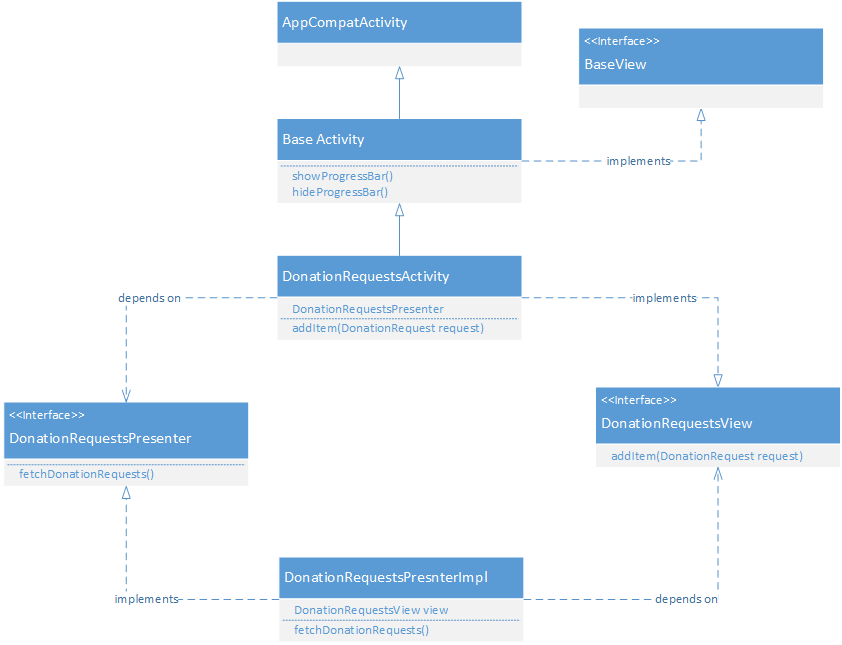
\includegraphics[width=1.1\textwidth]{android_mvp_example_class_diagram.png}
	    \caption{Παράδειγμα διαγράμματος κλάσεων - MVP Android.}
	    \label{fig:android_mvp_example_class_diagram}
	\end{figure}
	
	Σε αυτό το σημείο πρέπει να σημειωθεί ότι για το dependency injection που φαίνεται στο σχήμα \ref{fig:android_mvp_example_class_diagram} έγινε χρήση του dependency injector dagger\cite{daggerAndroid}. 
	
   		\subsubsection{Σύνδεση στην εφαρμογή - Login}
   		
   		Η οθόνη σύνδεσης στο σύστημα υλοποιείται μέσω ενός LoginActivity και ενός LoginPresenter ο οποίος το συνοδεύει. Όπως δείξαμε και στο σχήμα \ref{fig:android_mvp_example_class_diagram}, ο LoginPresenter γίνεται inject στο LoginActivity και το LoginView (το οποίο υλοποιείται από το LoginActivity) γίνεται inject στον LoginPresenter αντίστοιχα. Μόλις ο χρήστης συμπληρώσει τα στοιχεία του και κάνει tap στο κουμπί σύνδεσης, το LoginActivity ``περνάει" τα διαπιστευτήρια στον LoginPresenter ο οποίος αρχικώς τα ελέγχει για να εξακριβώσει την ορθότητα τους. Σε περίπτωση προβλήματος ως προς την ορθότητα ο LoginPresenter λέει στο LoginActivity τι μήνυμα λάθους θα πρέπει να δείξει στον χρήστη. Σε περίπτωση που δεν υπάρχει πρόβλημα ορθότητας, επικοινωνεί με το μοντέλο για να κάνει ταυτοποίηση του χρήστη. Τέλος ο LoginPresenter ενημερώνει το LoginActivity το οποίο με την σειρά του ενημερώνει τον χρήστη με κατάλληλο μήνυμα. 
   		
   		Παρακάτω βλέπουμε ενδεικτικά την κλήση του Presenter από το Activity:
   		\lstinputlisting[language=Java]{attempt_login.java}
		
		Παρακάτω βλέπουμε ενδεικτικά πως ο Presenter λέει στο Activity να δείξει μήνυμα λάθους:
		\lstinputlisting[language=Java]{loginPresenter_error.java}



\subsection{Εγγραφή στην εφαρμογή - Sign Up}	

		

   		Η οθόνη εγγραφής στο σύστημα υλοποιείται μέσω ενός RegisterActivity και ενός RegisterPresenter ο οποίος το συνοδεύει. Ο RegisterPresenter γίνεται inject στο RegisterActivity και το RegisterView (το οποίο υλοποιείται από το RegisterActivity) γίνεται inject στον RegisterPresenter αντίστοιχα. Μόλις ο χρήστης συμπληρώσει τα απαραιτητά για την εγγραφή του στοιχεία (ΑΜΚΑ) και κάνει tap στο κουμπί εγγραφής, το RegisterActivity καλεί τον RegisterPresenter ο οποίος αρχικώς τα ελέγχει για να εξακριβώσει την ορθότητα τους. Με βάση τα στοιχεία εγγραφής, ανοίγει ασφαλή δίαυλο επικοινωνίας με τη βάση δεδομένων της ΗΔΙΚΑ και "τραβάει" τα στοιχεία του χρήστη και στην συνέχεια επικοινωνεί με το κατάλληλο model, το οποίο θα περάσει τα στοιχεία στην βάση δεδομένων στο υπολογιστικό νέφος (cloud computing). Τέλος, ο RegisterPresenter λέει στο RegisterActivity να εμφανίσει το κατάλληλο μήνυμα στον χρήστη.
   
   		
   		Παρακάτω βλέπουμε ενδεικτικά την κλήση του Presenter από το Activity:
   			
   			
   				\begin{lstlisting}[language=Java]			
		
    @OnClick(R.id.register_button)
    protected void attemptRegister()
    {
        resetErrors();
        String AMKA = mAMKAlView.getText().toString().trim();
        registerPresenter.registerUser(AMKA);
    }
    
		\end{lstlisting}
		
		Παρακάτω βλέπουμε ενδεικτικά πως ο Presenter λέει στο Activity να δείξει ότι είχαμε επιτυχία:
	
	
   	\begin{lstlisting}[language=Java]			

	
	public void onSuccess()
    {
        view.navigateToFirstSignUp();
    }
    
    	\end{lstlisting}
	
	
\subsection{Δημιουργία νέου ραντεβού}	

	
   		Η οθόνη δημιουργίας ενός νέου ραντεβού στο σύστημα υλοποιείται μέσω ενός CreateAppointmentActivity και ενός CreateAppointmentPresenter ο οποίος το συνοδεύει. Ο CreateAppointmentPresenter γίνεται inject στο CreateAppointmentActivity και το CreateAppointmentView (το οποίο υλοποιείται από το CreateAppointmentActivity) γίνεται inject στον CreateAppointmentPresenter αντίστοιχα. O χρήστης βλέπει τα διαθέσιμα ραντεβού για ένα συγκεκριμένο γεγονός αιμοδοσίας και κάνοντας tap στην ώρα και ημέρα που επιθυμεί, του εμφανίζεται ένα μήνυμα επιβεβαίωσης της κράτησης του ραντεβού μέσω dialog fragment στο οποίο επιβεβαιώνει ή απορρίπτει την κράτηση του ραντεβού. Τα στοιχεία του ραντεβού μεταφέρονται από τον CreateAppointmentActivity στον CreateAppointmentPresenter ο οποίος αναλαμβάνει την κατοχύρωση του ραντεβού στο αιμοδοτικό κέντρο. Τέλος, ο CreateAppointmentPresenter λέει στο CreateAppointmentActivity να εμφανίσει το κατάλληλο μήνυμα στον χρήστη.
   
   		
   		Παρακάτω βλέπουμε ενδεικτικά την κλήση του Presenter από το Activity:
   			
   			
   	\begin{lstlisting}[language=Java]			
		
    @OnClick(R.id.create_appointment_button)
    protected void attemptCreateAppointment()
    {
        resetErrors();
        Date date = formatter.parse( date.getText().toString().trim() );
        Institution institution = Event.getInstitution();
        createAppointmentPresenter.createAppointment(institution,date,event);
    }
    
		\end{lstlisting}
		
\subsection{Εμφάνιση ιστορικού αιμοδοσιών}	

   		Η οθόνη εμφάνισης του ιστορικού αιμοδοσίας υλοποιείται μέσω ενός DonationsHistoryActivity και ενός DonationsHistoryPresenter ο οποίος το συνοδεύει. O χρήστης βλέπει μια λίστα από τις αιμοδοσίες τις οποίες έχει συμμετάσχει και έχει τη δυνατότητα με tap να δει επιπλέον πληροφορίες. 
   
   		Παρακάτω βλέπουμε ενδεικτικά την κλήση του Presenter από το Activity καθώς και την συνάρτηση που καλείται όταν ο χρήστης κάνει tap σε κάποια αιμοδοσία:
   			
   			
   	\begin{lstlisting}[language=Java]			
        donationRequestsPresenter.fetchDonationRequests(status);

        list.setOnItemClickListener(new AdapterView.OnItemClickListener()
        {
            @Override
            public void onItemClick(AdapterView<?> parent, View view, int position, long id)
            {
                Log.d(TAG,"Donation Request tapped,let's see the details");
                DonationRequest donationRequest = adapter.getItem(position);
                openDonationRequestDetailView(donationRequest);
            }
        });
		\end{lstlisting}
	 	 
	\subsection{Λήψη ειδοποίησης(push notification)}	

		Ο χρήστης λαμβάνει την ειδοποίηση (push notification), την ανοίγει και ξεκινά το DonationRequestDetailsActivity. Παρακάτω βλέπουμε ενδεικτικά την συνάρτηση που παίρνει τα δεδομένα από το push notification για να τα εμφανίσει στο DonationRequestActivity:
   			
   			
   	\begin{lstlisting}[language=Java]			
		
   public void updateView(final DonationRequest donationRequest)
    {
        if (donationRequest != null)
        {
            Event event = donationRequest.getEvent();
            String fullAddress = event.getStreet() + " " +event.getStreetNo();
            String fullBloodType = event.getBloodType() + event.getRhesus();
            String fullQuantity = event.getQuantity() + "/" + event.getQuantityRequired();

            venue.setText( event.getCity() );
            date.setText(event.getDate());
            address.setText(fullAddress);
            bloodType.setText(fullBloodType);
            quantity.setText(fullQuantity);
        }
    }
		\end{lstlisting}
	
	
		
	\section{Testing and Tools}
	
	\subsection{Android Application Testing}
	
	Στο παρόν κεφάλαιο θα αναφερθούμε αρχικά στο περιβάλλον ελέγχου που μας παρέχει το Android καθώς και στους διαφορετικού τύπους ελέγχου που μπορούμε να εκτελέσουμε. Στην συνέχεια θα αναφερθούμε στους ελέγχους που πραγματοποιήσαμε καθώς και στα αποτελέσματα τους.
	
	Η δυνατότητα αυτοματοποιημένου έλεγχου των εφαρμογών του λειτουργικού Android είναι ιδιαίτερα σημαντική λόγω του μεγάλου αριθμού διαφορετικών συσκευών που υπάρχουν στην αγορά. Είναι αδύνατον να δοκιμάσουμε για μία εφαρμογή όλες τις δυνατές ρυθμίσεις μιας συσκευής, για αυτό αποτελεί συνηθισμένη πρακτική η εκτέλεση δοκιμών με βάση τις πιο συνηθισμένες ρυθμίσεις. Στόχος είναι η επίτευξη ενός υψηλού ποσοστού κάλυψης δοκιμών (test coverage), έτσι ώστε να παράγουμε μια εφαρμογή απαλλαγμένη από σημαντικά σφάλματα αλλά και να διευκολύνουμε την συντήρηση και επέκτασή της στο μέλλον.
	
	Οι δοκιμές στο λειτουργικό σύστημα Android βασίζονται στο JUnit, και μπορούν να χωριστούν σε δύο μεγάλες κατηγορίες όπως φαίνεται στο σχήμα \ref{fig:categories_of_android_tests} ανάλογα με το αν απαιτούν το λειτουργικό συστήματα android ή αν χρειάζονται μόνο την εικονική μηχανή της Java (JVM - Java Virtual Machine) κατά την διάρκεια της εκτέλεσής τους\cite{androidTesting}.
	
	\begin{figure}[h]
	    \centering
	    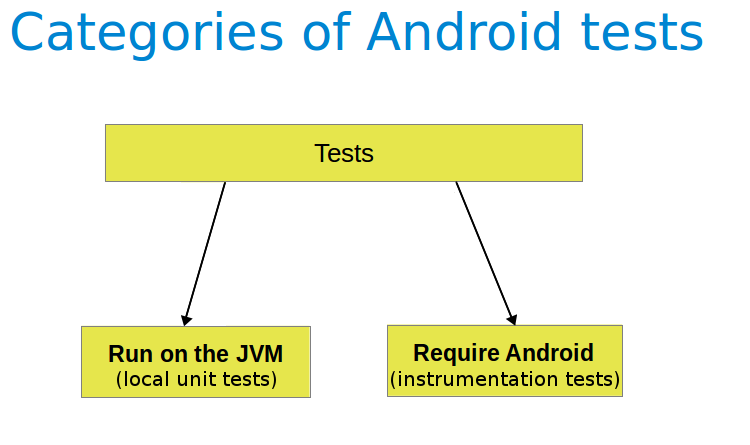
\includegraphics[width=0.7\textwidth]{categories_of_android_tests.png}
	    \caption{ Κατηγορίες δοκιμών στο Android}
	    \label{fig:categories_of_android_tests}
	\end{figure}
	
	Εφόσον είναι εφικτό, είναι πάντα προτιμότερο να τρέχουμε τις δοκιμές στην εικονική μηχανή της Java, δεδομένου ότι απαιτεί πολύ λιγότερο χρόνο σε σχέση με το χρόνο που απαιτείται για την εγκατάσταση και εκτέλεση της εφαρμογής σε μία συσκευή Android. Στην συνέχεια της παρούσας ενότητας η εφαρμογή που δοκιμάζεται θα αποκαλείται \textit{εφαρμογή υπό δοκιμή}.
	
		\subsubsection{Unit Testing (Δοκιμή μονάδας)}
		Έλεγχοι τύπου unit testing χρησιμοποιούνται για την δοκιμή μικρών μεμονωμένων στοιχείων της εφαρμογής, χωρίς να εξετάζεται η αλληλεπίδραση τους με άλλα στοιχεία της εφαρμογής. Δηλαδή όπως δηλώνει και το όνομα τους, εξετάζουν τη συμπεριφορά ενός στοιχείου ως ξεχωριστή μονάδα. Για να γίνει καλύτερα αντιληπτό το παραπάνω, ας υποθέσουμε ότι θέλουμε να δοκιμάσουμε ένα κουμπί το οποίο αναμένουμε να μας μεταφέρει σε μια άλλη οθόνη.  Στα πλαίσια της δοκιμής μονάδας θα γίνει έλεγχος αν η πρόθεση (intent) για αλλαγή οθόνης δημιουργήθηκε σωστά και όχι αν μεταφερθήκαμε στην άλλη οθόνη. Σε περίπτωση όμως που εκτελούσαμε δοκιμές ενσωμάτωσης (instrumentation testing βλ. ενότητα \ref{sssec:instrumentation_testing}) θα έπρεπε να γίνει έλεγχος ότι η επόμενη οθόνη ξεκίνησε όπως αναμέναμε.
		
		Τα Unit tests χρησιμοποιούν το JUnit test framework και δεν πρέπει να χρησιμοποιούν λειτουργίες από το Android API έτσι ώστε να είναι σε θέση να τρέξουν στην εικονική μηχανή της Java (JVM) κάτι το οποίο απαιτεί πολύ λιγότερο χρόνο σε σχέση με τον χρόνο τον οποίο θα χρειάζονταν για να τρέξουν σε περιβάλλον Android. Κάθε εξάρτηση από το λειτουργικό Android θα πρέπει να αντικατασταθεί στον κώδικα που θέλουμε να δοκιμάσουμε με κάποιο mocking framework όπως είναι το Mockito. 
		
		Παρακάτω βλέπουμε ένα απλό JUnit test που φτιάξαμε με σκοπό να δοκιμάσουμε την λειτουργία της συνάρτησης που ελέγχει την εγκυρότητα του κωδικού χρήστη.
		
		\lstinputlisting[language=Java]{ValidatorTest.java}  

		\subsubsection{Instrumentation Testing}\label{sssec:instrumentation_testing}

		Όταν θέλουμε να δοκιμάσουμε κλάσεις και λειτουργίες της εφαρμογής οι οποίες αλληλεπιδρούν με το λειτουργικό Android τότε δημιουργούμε τις λεγόμενες δοκιμές ενσωμάτωσης (instrumentation tests). Το Android API για δοκιμές παρέχει στον προγραμματιστή άγκιστρα (hooks) μέσω των οποίων μπορεί να αλληλεπιδράσει με τον κύκλο ζωής των στοιχείων λογισμικού και της εφαρμογής. Αυτά τα άγκιστρα απαρτίζουν το instrumentation API και επιτρέπουν στις δοκιμές να ελέγχουν γεγονότα από τον κύκλο ζωής (life cycle events) και την αλληλεπίδραση του χρήστη.

		Υπό κανονικές συνθήκες ένα στοιχείο του Android ακολουθεί έναν κύκλο ζωής που έχει καθοριστεί από το σύστημα βάση της αλληλεπίδρασης του με τον χρήστη. Για παράδειγμα, όταν δημιουργείται μια πρόθεση (intent) για έναρξη κάποιου Activity, καλείται η μέθοδος onCreate() του εν λόγω Activity. Στην συνέχεια αν ο χρήστης ανοίξει κάποια άλλη εφαρμογή, καλείται η μέθοδος onDestroy() του Activity . Το instrumentation API αν και δεν επιτρέπει στον προγραμματιστή να καλέσει αυτές τις μεθόδους απευθείας, του επιτρέπει να εξομοιώσει πλήρως την συμπεριφορά ενός χρήστη η οποία προκαλεί τέτοια γεγονότα. Για παράδειγμα επιτρέπει στον προγραμματιστή να στείλει γεγονότα πλήκτρων ή αφής, ελέγχοντας με αυτό τον τρόπο τον κύκλο ζωής της υπό δοκιμής εφαρμογής\cite{androidTestingBook}.

		Τα instrumentation tests δεν γίνεται να τρέξουν στο JVM αλλά χρειάζονται περιβάλλον με λειτουργικό σύστημα Android. Μπορούν να τρέξουν είτε σε πραγματική συσκευή Android η οποία έχει συνδεθεί με τον υπολογιστή στον οποίο γίνεται η ανάπτυξη, είτε σε εικονική συσκευή Android. Δεδομένου του πλήθους των συσκευών που τρέχουν το λειτουργικό σύστημα Android, και συνυπολογίζοντας τις διάφορες εκδόσεις που μπορεί να τρέχει κάθε συσκευή, κάθε δοκιμή θα πρέπει να γίνεται με χρήση εξομοίωσης σε διάφορα επίπεδα API αλλά και μεγέθη οθονών. Για παράδειγμα αν η εφαρμογή υποστηρίζει επίπεδο API μεγαλύτερο του 14 θα πρέπει να γίνει έλεγχος για κάθε API μεγαλύτερο του 14 με τουλάχιστον 2 διαφορετικά μεγέθη οθόνης για κάθε API. 
		
		Όπως γίνεται εμφανές από τα παραπάνω το τρέξιμο των instrumentation tests αποτελεί μια ιδιαίτερα χρονοβόρα διαδικασία. Για την εξομάλυνση αυτού του προβλήματος υπάρχουν υπηρεσίες μέσω των οποίων οι δοκιμές μπορούν να γίνουν στο υπολογιστικό νέφος. Παρακάτω βλέπουμε ένα παράδειγμα δοκιμών instrumentation που φτιάξαμε για να ελέγξουμε την λειτουργία επαναφοράς κωδικού.
		
		\lstinputlisting[language=Java]{ResetPassword.java}
		
		\subsection{NodeJs Testing}
		
		
		Για τη συγγραφή και εκτέλεση τεστ για τον κώδικα σε JavaScript χρησιμοποιήσαμε τα εργαλεία Karma και Mocha.Το Mocha είναι μια βιβλιοθήκη που επιτρέπει τον ορισμό και την εκτέλεση δοκιμών σε ένα περιβάλλον Node.js χωρίς την ανάγκη ύπαρξης ενός φυλλομετρητή. Ορίζει περισσότερα από ένα στυλ συγγραφής τεστ και μας επιτρέπει να επιλέξουμε εκείνο που ταιριάζει περισσότερο στις ανάγκες του εκάστοτε τεστ. Στην περίπτωση που θέλουμε τα τεστ να εκτελούνται σε φυλλομετρητή το Mocha μας επιτρέπει να φορτώσουμε τα τεστ σε μία HTML σελίδα και να τα εκτελέσουμε στο φυλλομετρητή.
		
		
		Το Chai είναι μία βιβλιοθήκη επικυρώσεων (assertion framework), η οποία συνεργάζεται άψογα με τη βιβλιοθήκη Mocha και δίνει τη δυνατότητα ορισμού των αναμενόμενων αποτελεσμάτων από κάποιο τεστ και ελέγχου κατά την εκτέλεσή του. Επίσης, όπως και το Mocha, μας επιτρέπει να διαλέξουμε από ένα σύνολο διαφορετικών στυλ για τον ορισμό των προσδοκιών. Παρατίθεται παράδειγμα τεστ γραμμένου με χρήση mocha και chai.
		
		\begin{lstlisting}[language=JavaScript]		
		describe('JavaScript', function()){
		it('should perform substraction properly', function() 
		{
	     expect(2 - 0).to.equal(2);
		expect(5 - 2).to.equal(3); 
		expect(7 - 3).not.to.equal(4);
		}); 
		});
				\end{lstlisting}
				
				Τέλος, το Karma είναι ένα εργαλείο το οποίο ενώνει τις δυνατότητες των ανωτέρω βιβλιοθηκών σε μία σελίδα HTML, εκτελεί όλα τα τεστ και επιστρέφει τα αποτελέσματα από την εκτέλεσή τους. Το Karma, βασίζεται σε ένα αρχείο ρυθμίσεων με βάση το οποίο γνωρίζει ποιες βιβλιοθήκες να χρησιμοποιήσει, που να βρει τα τεστ, σε τι πρόγραμμα περιήγησης να τα εκτελέσει, πώς να δημοσιεύσει τα αποτελέσματα και ενδεχομένως επιπλέον πληροφορίες σχετικές με την εκτέλεση των τεστ. 


